\documentclass[../Interim_Report_Master]{subfiles}
\begin{document}
\begin{landscape}
\hypertarget{proj_plan}{\section*{Project Plan}\label{proj_plan}}
Progress against the project plan is shown in Figure \ref{Gantt_Chart}. Implementing the models in the Python code has taken longer than expected, as has the literature review process. The main unknown unknown was getting the coupled heat and mass transfer working, which has been achieved. With results matching those found in the literature. Little has been done on evaluating the previous code. Although the author has taken the time to read through and understand the relevant parts of the previous Python implementation. 

A risk identified at the start of the project was the timetabling of modules between semester 1 and semester 2. The author only has two modules in semester 2 affording much more time on producing results now that working code has been developed.

\vspace*{\fill}
\begin{figure}[h]
	\centering
	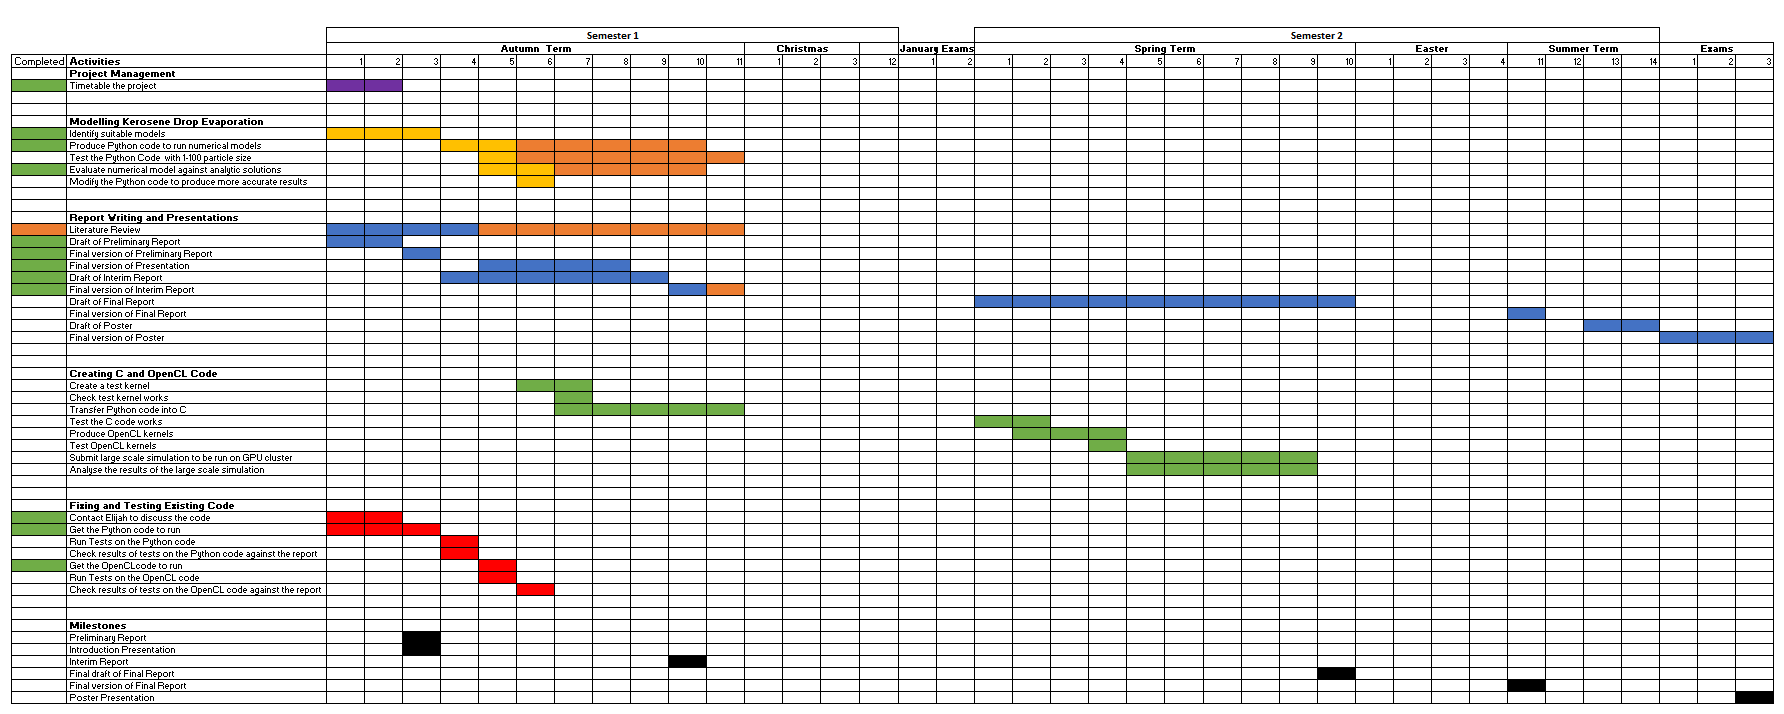
\includegraphics[width=1.4\textwidth]{Gantt_Chart_Updated_2.png}
	\caption{Project Gantt Chart.}
	\label{Gantt_Chart}
\end{figure}
\vfill
\end{landscape}
\end{document}